%%%%%%%%%%%%%%%%%%%%%%%%%%%%%%%%%%%%%%%%%
% Beamer Presentation
% LaTeX Template
% Version 1.0 (10/11/12)
%
% This template has been downloaded from:
% http://www.LaTeXTemplates.com
%
% License:
% CC BY-NC-SA 3.0 (http://creativecommons.org/licenses/by-nc-sa/3.0/)
%
%%%%%%%%%%%%%%%%%%%%%%%%%%%%%%%%%%%%%%%%%

%----------------------------------------------------------------------------------------
%	PACKAGES AND THEMES
%----------------------------------------------------------------------------------------

\documentclass{beamer}

\mode<presentation> {

% The Beamer class comes with a number of default slide themes
% which change the colors and layouts of slides. Below this is a list
% of all the themes, uncomment each in turn to see what they look like.

%\usetheme{default}
%\usetheme{AnnArbor}
%\usetheme{Antibes}
%\usetheme{Bergen}
%\usetheme{Berkeley}
%\usetheme{Berlin}
\usetheme{Boadilla}
%\usetheme{CambridgeUS}
%\usetheme{Copenhagen}
%\usetheme{Darmstadt}
%\usetheme{Dresden}
%\usetheme{Frankfurt}
%\usetheme{Goettingen}
%\usetheme{Hannover}
%\usetheme{Ilmenau}
%\usetheme{JuanLesPins}
%\usetheme{Luebeck}
%\usetheme{Madrid}
%\usetheme{Malmoe}
%\usetheme{Marburg}
%\usetheme{Montpellier}
%\usetheme{PaloAlto}
%\usetheme{Pittsburgh}
%\usetheme{Rochester}
%\usetheme{Singapore}
%\usetheme{Szeged}
%\usetheme{Warsaw}

% As well as themes, the Beamer class has a number of color themes
% for any slide theme. Uncomment each of these in turn to see how it
% changes the colors of your current slide theme.

\setbeamercolor{normal text}{fg=white, bg=black}


%\usecolortheme{albatross}
\usecolortheme{beaver}
%\usecolortheme{beetle}
%\usecolortheme{crane}
%\usecolortheme{dolphin}
%\usecolortheme{dove}
%\usecolortheme{fly}
%\usecolortheme{lily}
%\usecolortheme{orchid}
%\usecolortheme{rose}
%\usecolortheme{seagull}
%\usecolortheme{seahorse}
%\usecolortheme{whale}
%\usecolortheme{wolverine}

%\setbeamertemplate{footline} % To remove the footer line in all slides uncomment this line
%\setbeamertemplate{footline}[page number] % To replace the footer line in all slides with a simple slide count uncomment this line

%\setbeamertemplate{navigation symbols}{} % To remove the navigation symbols from the bottom of all slides uncomment this line
}

\usepackage{graphicx} % Allows including images
\usepackage{booktabs} % Allows the use of \toprule, \midrule and \bottomrule in tables

%adding video package
\usepackage{media9}
\usepackage[utf8]{inputenc}
\usepackage[T1]{fontenc}
\usepackage{parskip}
%\usepackage{multimedia}
\usepackage{pdfpc-commands}
%----------------------------------------------------------------------------------------
%	TITLE PAGE
%----------------------------------------------------------------------------------------

\title[Detonation Initiation]{Turbulently-Driven Detonation Initiation in Electron-Degenerate Matter} % The short title appears at the bottom of every slide, the full title is only on the title page

\author{Gabriel Casabona} % Your name
\institute[UMassD] % Your institution as it will appear on the bottom of every slide, may be shorthand to save space
{
University of Massachusetts Dartmouth \\ % Your institution for the title page
\medskip
\textit{MS Thesis Defense} % Your email address
}
\date{\today} % Date, can be changed to a custom date

\begin{document}

\begin{frame}
\titlepage % Print the title page as the first slide
\end{frame}

%\begin{frame}
%\frametitle{Overview} % Table of contents slide, comment this block out to remove it
%\tableofcontents % Throughout your presentation, if you choose to use \section{} and \subsection{} commands, these will automatically be printed on this slide as an overview of your presentation
%\end{frame}

%----------------------------------------------------------------------------------------
%	PRESENTATION SLIDES
%----------------------------------------------------------------------------------------

%------------------------------------------------
\section{First Section} % Sections can be created in order to organize your presentation into discrete blocks, all sections and subsections are automatically printed in the table of contents as an overview of the talk
%------------------------------------------------

\subsection{Subsection Example} % A subsection can be created just before a set of slides with a common theme to further break down your presentation into chunks

%\begin{frame}
%\frametitle{Paragraphs of Text}
%Sed iaculis dapibus gravida. Morbi sed tortor erat, nec interdum arcu. Sed id lorem lectus. Quisque viverra augue id sem ornare non aliquam nibh tristique. Aenean in ligula nisl. Nulla sed tellus ipsum. Donec vestibulum ligula non lorem vulputate fermentum accumsan neque mollis.\\~\\

%Sed diam enim, sagittis nec condimentum sit amet, ullamcorper sit amet libero. Aliquam vel dui orci, a porta odio. Nullam id suscipit ipsum. Aenean lobortis commodo sem, ut commodo leo gravida vitae. Pellentesque vehicula ante iaculis arcu pretium rutrum eget sit amet purus. Integer ornare nulla quis neque ultrices lobortis. Vestibulum ultrices tincidunt libero, quis commodo erat ullamcorper id.
%\end{frame}

%------------------------------------------------

\begin{frame}
\frametitle{Type Ia Supernova}

\begin{columns}[c]
        \column{0.5\textwidth}
	\begin{itemize}
		\item Strong Silicon lines in the absence of Hydrogen
		\item Used as standardizable candles
		\item Led to the discovery of the accelerated expansion of the universe
		\item Cosmic Rays
	\end{itemize}

\end{figure}

\column{0.5\textwidth}
        \begin{figure}
    \begin{center}
      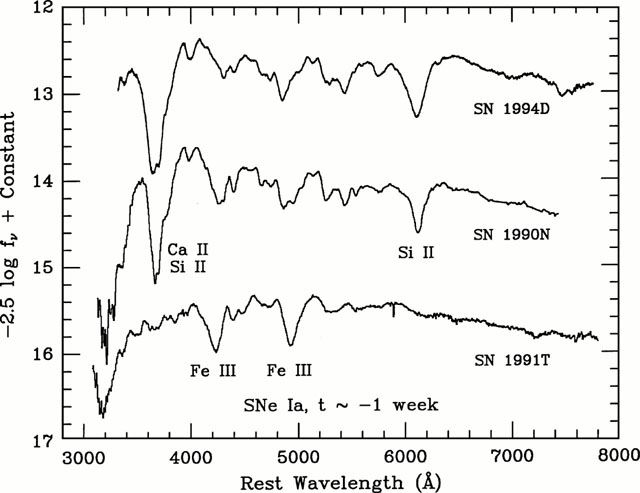
\includegraphics[width=.90\linewidth]{spectrum.jpg}
	    \caption{Fillipenko}
    \end{center}
  \end{figure}

        \end{columns}

\end{frame}


%------------------------------------------------

\begin{frame}
	
	\frametitle{movie}
	\begin{center}
	\inlineMovie[loop&autostart]{out.mp4}{out.png}{height=0.7\textheight}
	\end{center}
	\caption{caption}
\end{frame}






\end{document}
